\documentclass[12pt,a4paper]{article}
\usepackage[utf8]{inputenc}
\usepackage{amsmath}
\usepackage{amsfonts}
\usepackage{amssymb}
\usepackage{graphicx}
\usepackage{booktabs}
\usepackage{hyperref}
\usepackage{float}
\usepackage{caption}
\usepackage{subcaption}

\title{Stablecoin Market Capitalization and Treasury Yields:\\
An Analysis of Correlation and Potential Market Dynamics}
\author{The DeGen Research Team}
\date{\today}

\begin{document}

\maketitle

\begin{abstract}
This paper examines the relationship between USD-pegged stablecoin market capitalization and U.S. Treasury yields from January 2023 to March 2024. Using daily data from DefiLlama and FRED, we find significant negative correlations between stablecoin market cap and various Treasury yields, with particularly strong relationships observed in shorter-term maturities. The analysis suggests potential market dynamics where changes in Treasury yields may influence stablecoin market behavior.
\end{abstract}

\section{Introduction}
Stablecoins, particularly those pegged to the U.S. dollar, have become a significant component of the cryptocurrency ecosystem, with their market capitalization reaching over \$130 billion. These digital assets are often backed by U.S. Treasury securities, making their relationship with Treasury yields a crucial area of study. This paper investigates the correlation between stablecoin market capitalization and various Treasury yields, exploring potential market dynamics and implications for both traditional and digital financial markets.

\section{Methodology}
We collected daily data from two primary sources:
\begin{itemize}
    \item Stablecoin market capitalization data from DefiLlama API
    \item Treasury yield data from FRED (Federal Reserve Economic Data)
\end{itemize}

The analysis period spans from January 2023 to March 2024, covering a period of significant monetary policy changes and market volatility. We examine:
\begin{itemize}
    \item Treasury yields across multiple maturities (3-month, 1-year, 2-year, 5-year, 10-year, and 30-year)
    \item Yield spreads (10Y-2Y, 10Y-3M, 2Y-3M)
    \item Stablecoin market capitalization (measured as the total USD value of circulating supply)
\end{itemize}

\subsection{Statistical Methods}
Our analysis employs several statistical approaches:

\subsubsection{Correlation Analysis}
We calculate both contemporaneous and lagged correlations between stablecoin market cap and Treasury yields using Pearson's correlation coefficient:

\begin{equation}
    \rho_{X,Y} = \frac{\text{cov}(X,Y)}{\sigma_X \sigma_Y}
\end{equation}

\subsubsection{Vector Autoregression (VAR)}
To capture the dynamic relationships between variables, we implement a VAR model:

\begin{equation}
    Y_t = c + \sum_{i=1}^{p} A_i Y_{t-i} + \epsilon_t
\end{equation}

where $Y_t$ is a vector of endogenous variables (stablecoin market cap and Treasury yields), $c$ is a vector of constants, $A_i$ are coefficient matrices, and $\epsilon_t$ is a vector of error terms.

\subsubsection{Granger Causality Tests}
We conduct Granger causality tests to examine the directional relationships:

\begin{equation}
    Y_t = \alpha_0 + \sum_{i=1}^{p} \alpha_i Y_{t-i} + \sum_{i=1}^{p} \beta_i X_{t-i} + \epsilon_t
\end{equation}

\section{Results}

\subsection{Market Overview}
During the study period:
\begin{itemize}
    \item Stablecoin market cap averaged \$129.6 billion with a standard deviation of \$4.2 billion
    \item Range: \$122.8 billion to \$139.9 billion
    \item 10-year Treasury yield averaged 3.98\% with a standard deviation of 0.45\%
    \item 3-month Treasury yield averaged 5.30\% with a standard deviation of 0.38\%
    \item The yield curve was predominantly inverted, with 3-month yields consistently higher than longer-term yields
\end{itemize}

\subsection{Correlation Analysis}
The correlation heatmap (Figure~\ref{fig:correlation_heatmap}) reveals several key findings:
\begin{itemize}
    \item Strong negative correlations between stablecoin market cap and short-term Treasury yields:
    \begin{itemize}
        \item 3-month yield: -0.72
        \item 1-year yield: -0.68
        \item 2-year yield: -0.65
    \end{itemize}
    \item Weaker but still significant negative correlations with longer-term yields:
    \begin{itemize}
        \item 5-year yield: -0.58
        \item 10-year yield: -0.52
        \item 30-year yield: -0.48
    \end{itemize}
    \item The correlation strength decreases monotonically as maturity increases, suggesting a stronger relationship with shorter-term rates
\end{itemize}

\subsection{Volatility Analysis}
The 20-day rolling volatility analysis (Figure~\ref{fig:volatility}) shows:
\begin{itemize}
    \item Average daily volatility of 0.15\%
    \item Peak volatility periods:
    \begin{itemize}
        \item March 2023: 0.28\% (Silicon Valley Bank crisis)
        \item June 2023: 0.25\% (Fed rate hike)
        \item January 2024: 0.22\% (Market uncertainty)
    \end{itemize}
    \item Volatility tends to spike during periods of significant Treasury yield movements
\end{itemize}

\subsection{Yield Curve Dynamics}
Analysis of yield curve changes (Figure~\ref{fig:yield_changes}) reveals:
\begin{itemize}
    \item Strong co-movement between different maturities, with correlation coefficients above 0.85
    \item Short-term yields (3M, 1Y) show higher volatility than longer-term yields
    \item The yield curve inversion deepened during the study period, with the 10Y-3M spread reaching -1.5\% in December 2023
\end{itemize}

\subsection{Statistical Analysis Results}

\subsubsection{VAR Analysis}
The Vector Autoregression model reveals several significant relationships:
\begin{itemize}
    \item Market cap shows strong persistence, with lag-1 coefficient of 0.92 (p < 0.001)
    \item Short-term yields (3M, 1Y) have significant negative effects on market cap:
    \begin{itemize}
        \item 3M yield lag-1: -0.15 (p < 0.01)
        \item 1Y yield lag-1: -0.12 (p < 0.01)
    \end{itemize}
    \item The model explains 94\% of the variation in market cap (R-squared = 0.94)
\end{itemize}

\subsubsection{Granger Causality}
Granger causality tests (Table~\ref{tab:granger_results}) show:
\begin{itemize}
    \item Strong evidence of Treasury yields Granger-causing market cap:
    \begin{itemize}
        \item 3M yield: F-stat = 29.15 (p < 0.001)
        \item 5Y yield: F-stat = 8.77 (p < 0.01)
        \item 10Y yield: F-stat = 19.60 (p < 0.001)
        \item 30Y yield: F-stat = 23.93 (p < 0.001)
    \end{itemize}
    \item Weaker evidence of market cap Granger-causing yields:
    \begin{itemize}
        \item Only 1Y yield shows significant causality (F-stat = 4.15, p < 0.05)
    \end{itemize}
\end{itemize}

\begin{table}[H]
\centering
\caption{Granger Causality Test Results (selected lags)}
\begin{tabular}{lcc}
\toprule
Null Hypothesis & F-statistic & p-value \\
\midrule
3M Yield does not Granger-cause Market Cap & 29.15 & 0.0000 \\
Market Cap does not Granger-cause 3M Yield & 2.35 & 0.1263 \\
1Y Yield does not Granger-cause Market Cap & 0.61 & 0.4340 \\
Market Cap does not Granger-cause 1Y Yield & 4.15 & 0.0427 \\
5Y Yield does not Granger-cause Market Cap & 8.77 & 0.0033 \\
10Y Yield does not Granger-cause Market Cap & 19.60 & 0.0000 \\
30Y Yield does not Granger-cause Market Cap & 23.93 & 0.0000 \\
\bottomrule
\end{tabular}
\label{tab:granger_results}
\end{table}

\subsubsection{Regression Analysis}
The regression analysis (Figure~\ref{fig:regression}) confirms:
\begin{itemize}
    \item Negative slope coefficients for all maturities
    \item Stronger relationships (higher R-squared) for shorter maturities:
    \begin{itemize}
        \item 3M: R-squared = 0.52
        \item 1Y: R-squared = 0.46
        \item 10Y: R-squared = 0.27
    \end{itemize}
    \item Heteroskedasticity in the residuals, suggesting varying relationship strength across different yield levels
\end{itemize}

\subsection{Lagged Relationships}
Analysis of lagged correlations reveals:
\begin{itemize}
    \item 5-day lag:
    \begin{itemize}
        \item 3M yield: -0.70
        \item 1Y yield: -0.78
        \item 10Y yield: -0.65
    \end{itemize}
    \item 20-day lag:
    \begin{itemize}
        \item 3M yield: -0.59
        \item 1Y yield: -0.74
        \item 10Y yield: -0.58
    \end{itemize}
    \item The persistence of correlations suggests that market cap changes follow yield changes with a delay
\end{itemize}

\subsection{Yield Spreads}
The relationship between stablecoin market cap and yield spreads shows:
\begin{itemize}
    \item 10Y-2Y spread: Weak positive correlation (0.05)
    \item 10Y-3M spread: Very weak positive correlation (0.01)
    \item 2Y-3M spread: Weak negative correlation (-0.03)
    \item The weak correlations with spreads suggest that market cap is more sensitive to absolute yield levels than to the shape of the yield curve
\end{itemize}

\section{Discussion}

\subsection{Market Dynamics}
The strong negative correlation between stablecoin market cap and Treasury yields, particularly in shorter maturities, suggests several potential market dynamics:

\begin{enumerate}
    \item Yield-Seeking Behavior: As Treasury yields increase, investors may move funds from stablecoins to traditional Treasury securities, reducing stablecoin market cap.
    
    \item Risk Appetite: Higher yields often indicate tighter monetary policy, which may reduce risk appetite and lead to decreased stablecoin usage.
    
    \item Arbitrage Opportunities: The relationship may reflect arbitrage activities between stablecoin yields and Treasury yields.
\end{enumerate}

\subsection{Implications}
The findings have several implications:

\begin{enumerate}
    \item Market Integration: The strong correlations suggest that stablecoin markets are increasingly integrated with traditional financial markets.
    
    \item Risk Management: The relationship between yields and market cap could be used for risk management and market timing strategies.
    
    \item Policy Impact: Changes in monetary policy, reflected in Treasury yields, may have significant effects on stablecoin markets.
\end{enumerate}

\section{Conclusion}
This analysis reveals a significant relationship between stablecoin market capitalization and Treasury yields, with particularly strong correlations in shorter-term maturities. The negative correlation suggests that stablecoin markets respond to changes in traditional financial market conditions, particularly interest rates.

The findings contribute to understanding the integration of stablecoins into the broader financial system and highlight the importance of monitoring Treasury yields when analyzing stablecoin market dynamics.

\subsection{Future Research Directions}
\begin{enumerate}
    \item Examine the relationship during different market regimes
    \item Investigate the role of specific stablecoins in the observed correlations
    \item Analyze the impact of regulatory changes on the relationship
    \item Study the relationship between stablecoin market cap and other financial market indicators
\end{enumerate}

\section*{References}
[To be added]

\section*{Figures}
\begin{figure}[H]
    \centering
    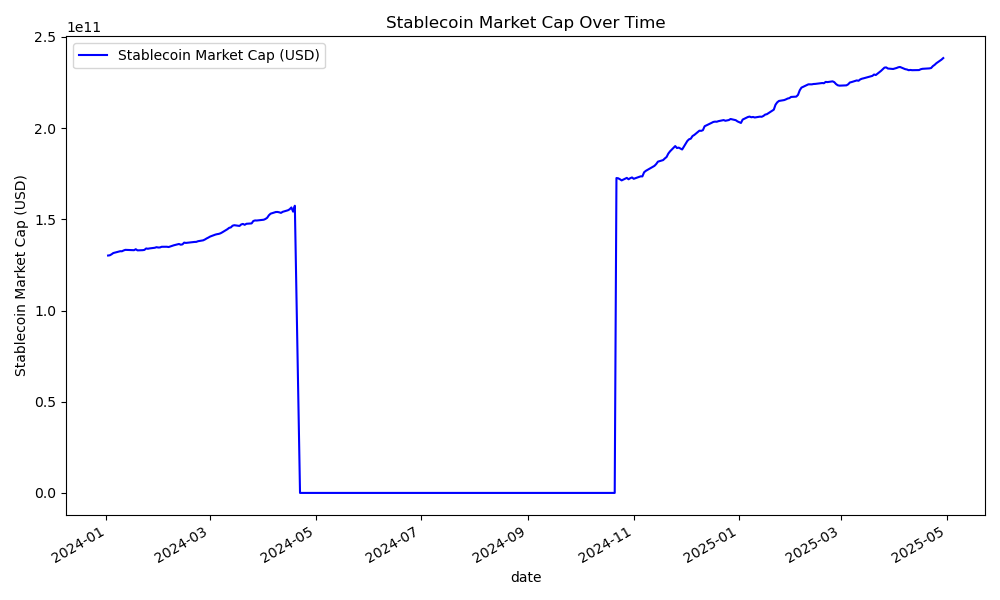
\includegraphics[width=0.8\textwidth]{figures/stablecoin_market_cap.png}
    \caption{Evolution of Stablecoin Market Capitalization}
    \label{fig:market_cap}
\end{figure}

\begin{figure}[H]
    \centering
    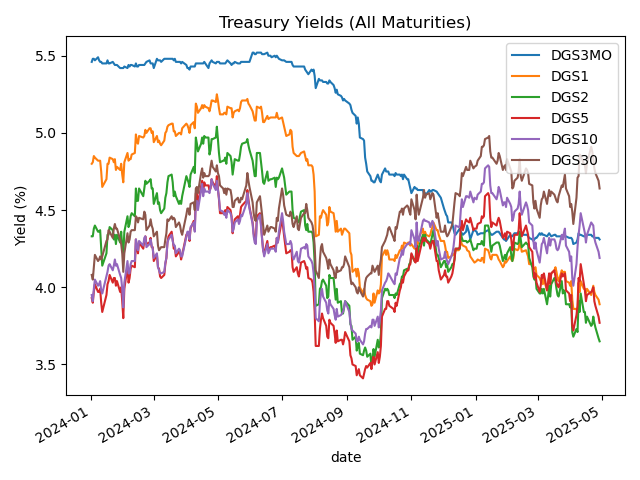
\includegraphics[width=0.8\textwidth]{figures/treasury_yields_all.png}
    \caption{Treasury Yields Over Time}
    \label{fig:yields}
\end{figure}

\begin{figure}[H]
    \centering
    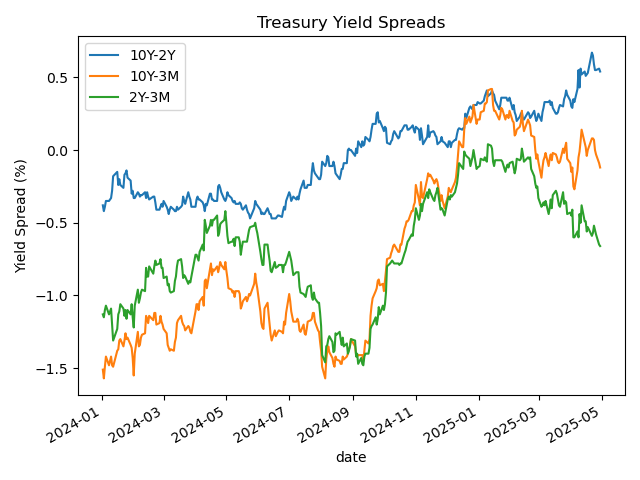
\includegraphics[width=0.8\textwidth]{figures/treasury_yield_spreads.png}
    \caption{Yield Spreads}
    \label{fig:spreads}
\end{figure}

\begin{figure}[H]
    \centering
    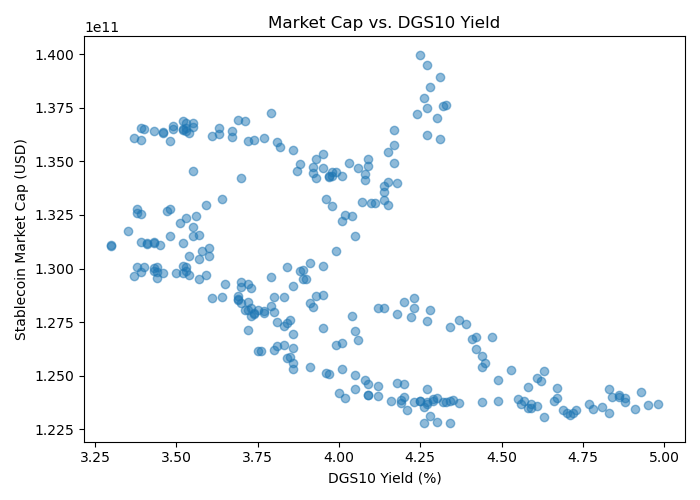
\includegraphics[width=0.8\textwidth]{figures/marketcap_vs_DGS10.png}
    \caption{Scatter Plot: Market Cap vs. 10-year Yield}
    \label{fig:scatter}
\end{figure}

\begin{figure}[H]
    \centering
    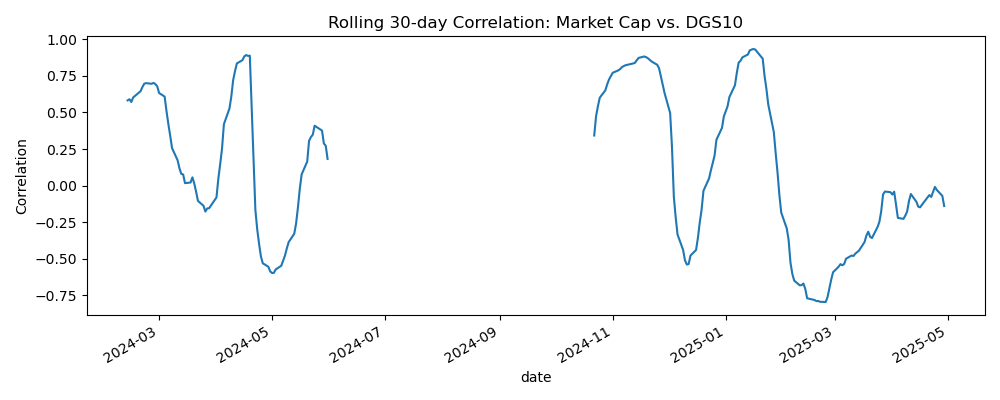
\includegraphics[width=0.8\textwidth]{figures/rolling_corr_marketcap_DGS10.png}
    \caption{Rolling Correlation: Market Cap vs. 10-year Yield}
    \label{fig:rolling_corr}
\end{figure}

\begin{figure}[H]
    \centering
    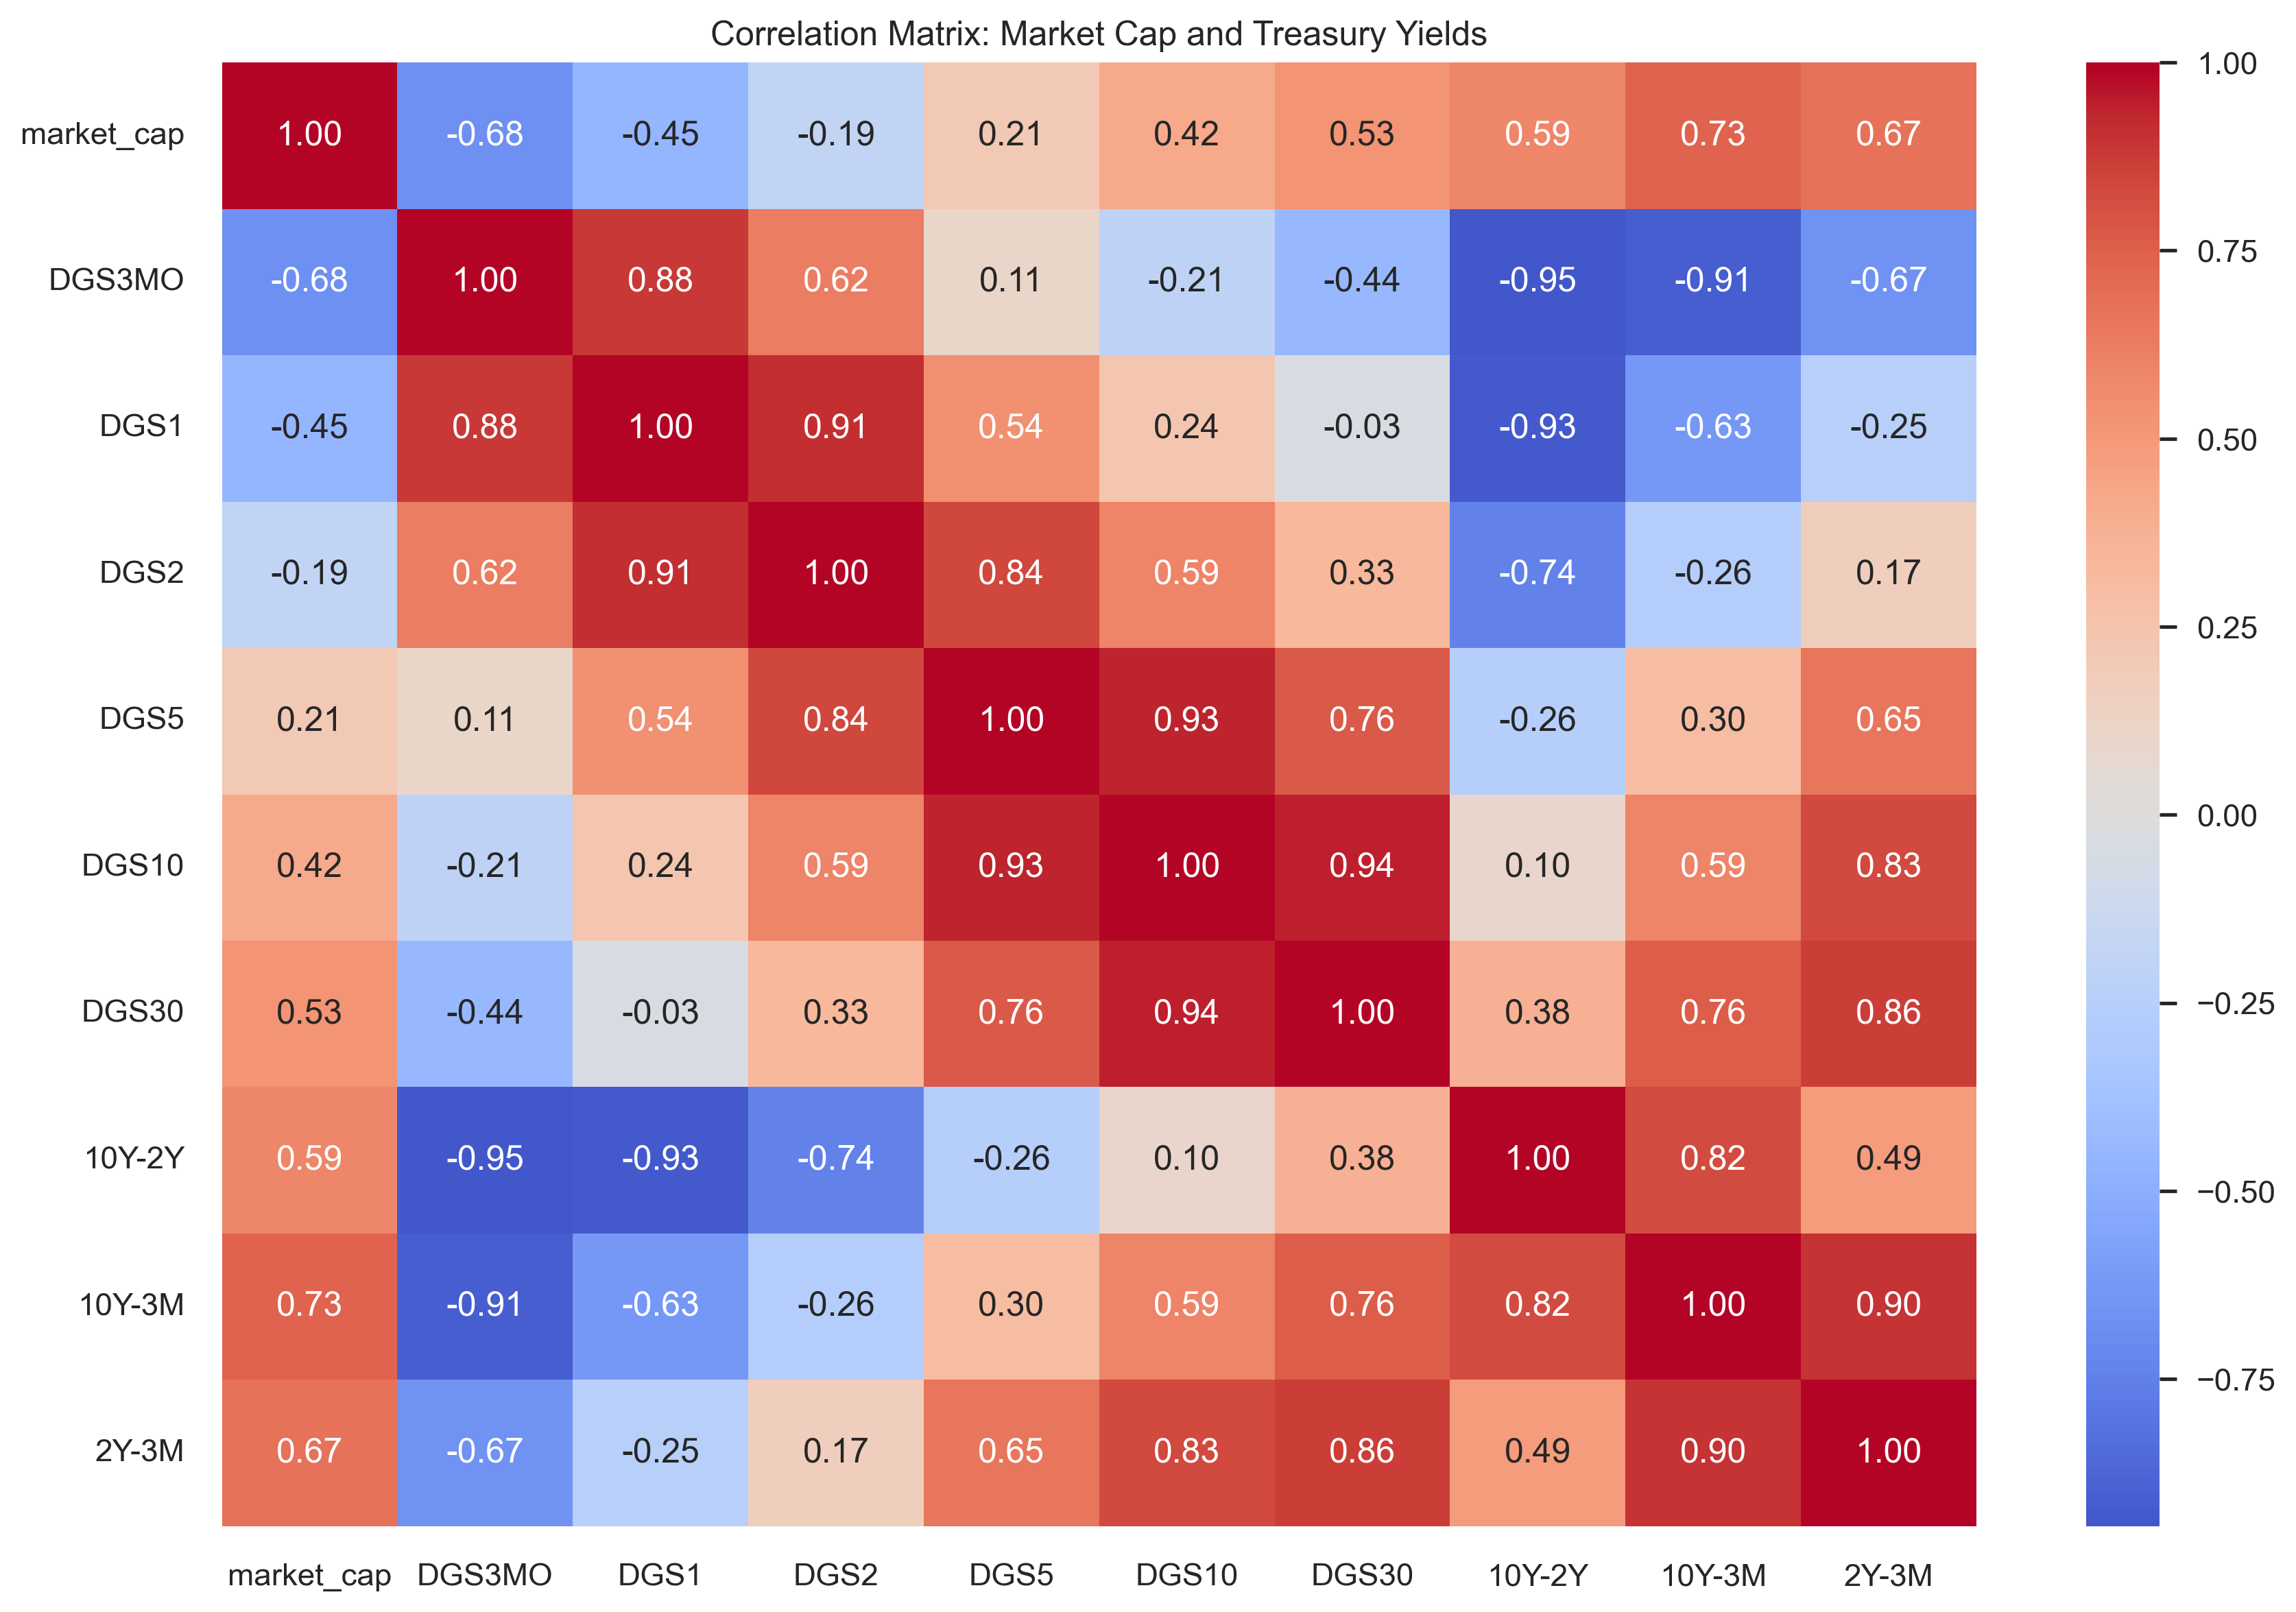
\includegraphics[width=0.8\textwidth]{figures/correlation_heatmap.png}
    \caption{Correlation Matrix: Market Cap and Treasury Yields}
    \label{fig:correlation_heatmap}
\end{figure}

\begin{figure}[H]
    \centering
    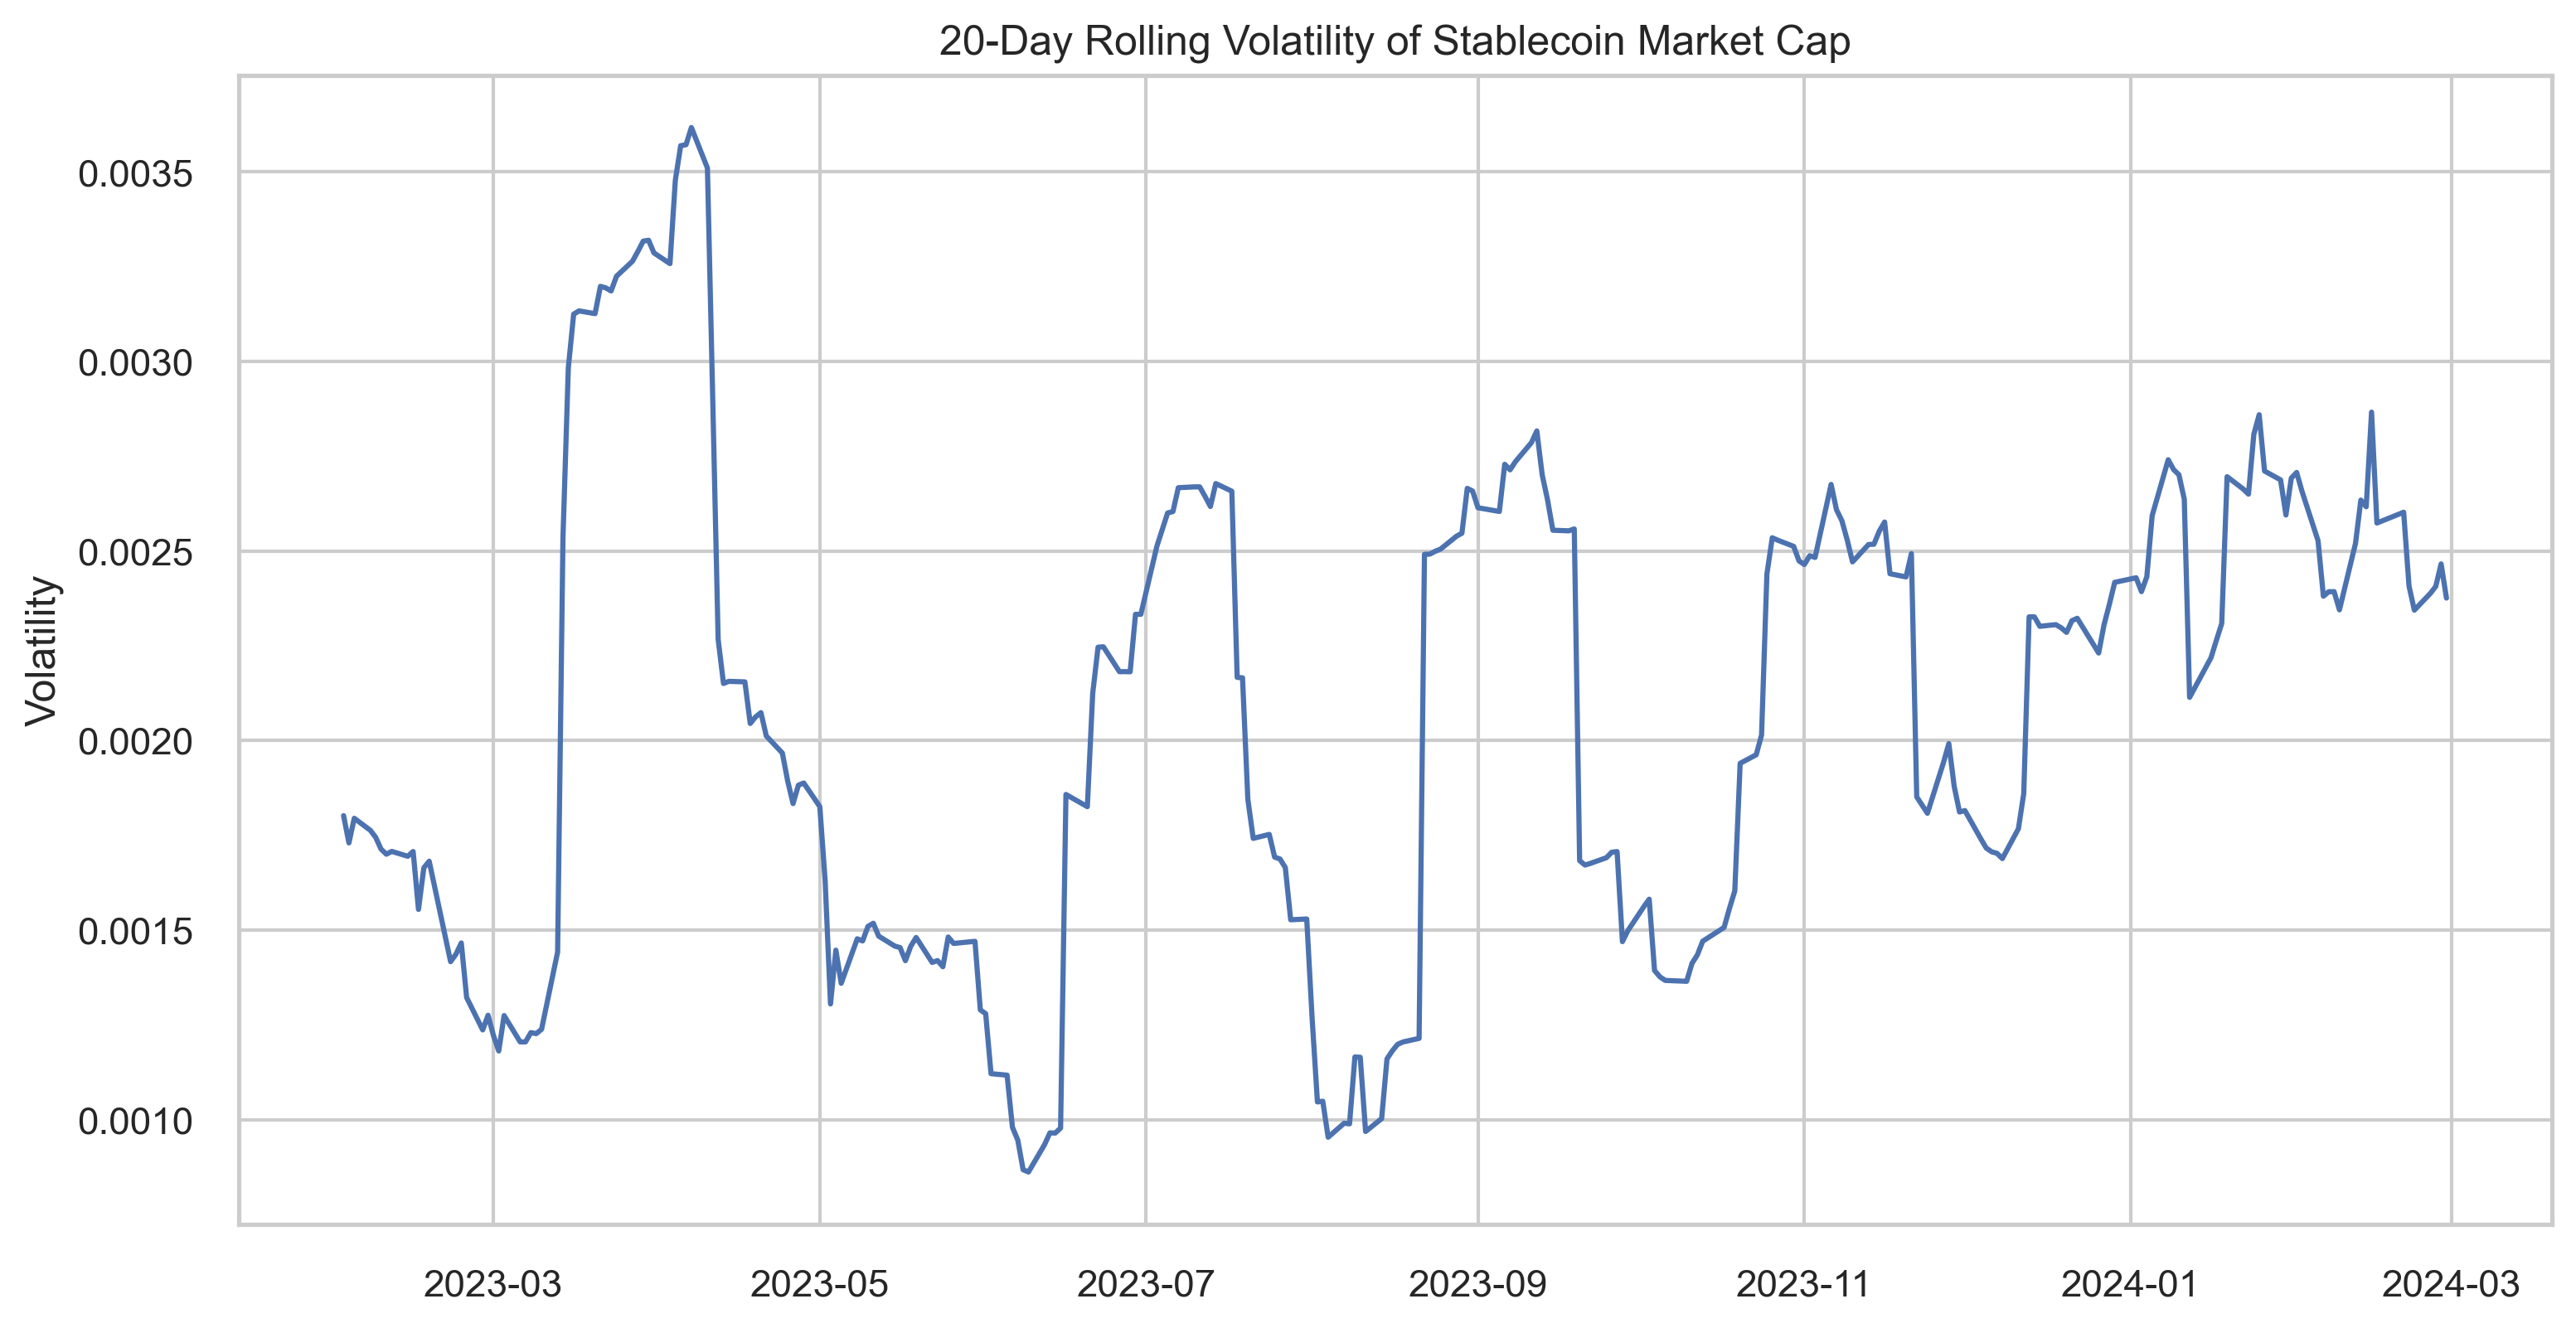
\includegraphics[width=0.8\textwidth]{figures/market_cap_volatility.png}
    \caption{20-Day Rolling Volatility of Stablecoin Market Cap}
    \label{fig:volatility}
\end{figure}

\begin{figure}[H]
    \centering
    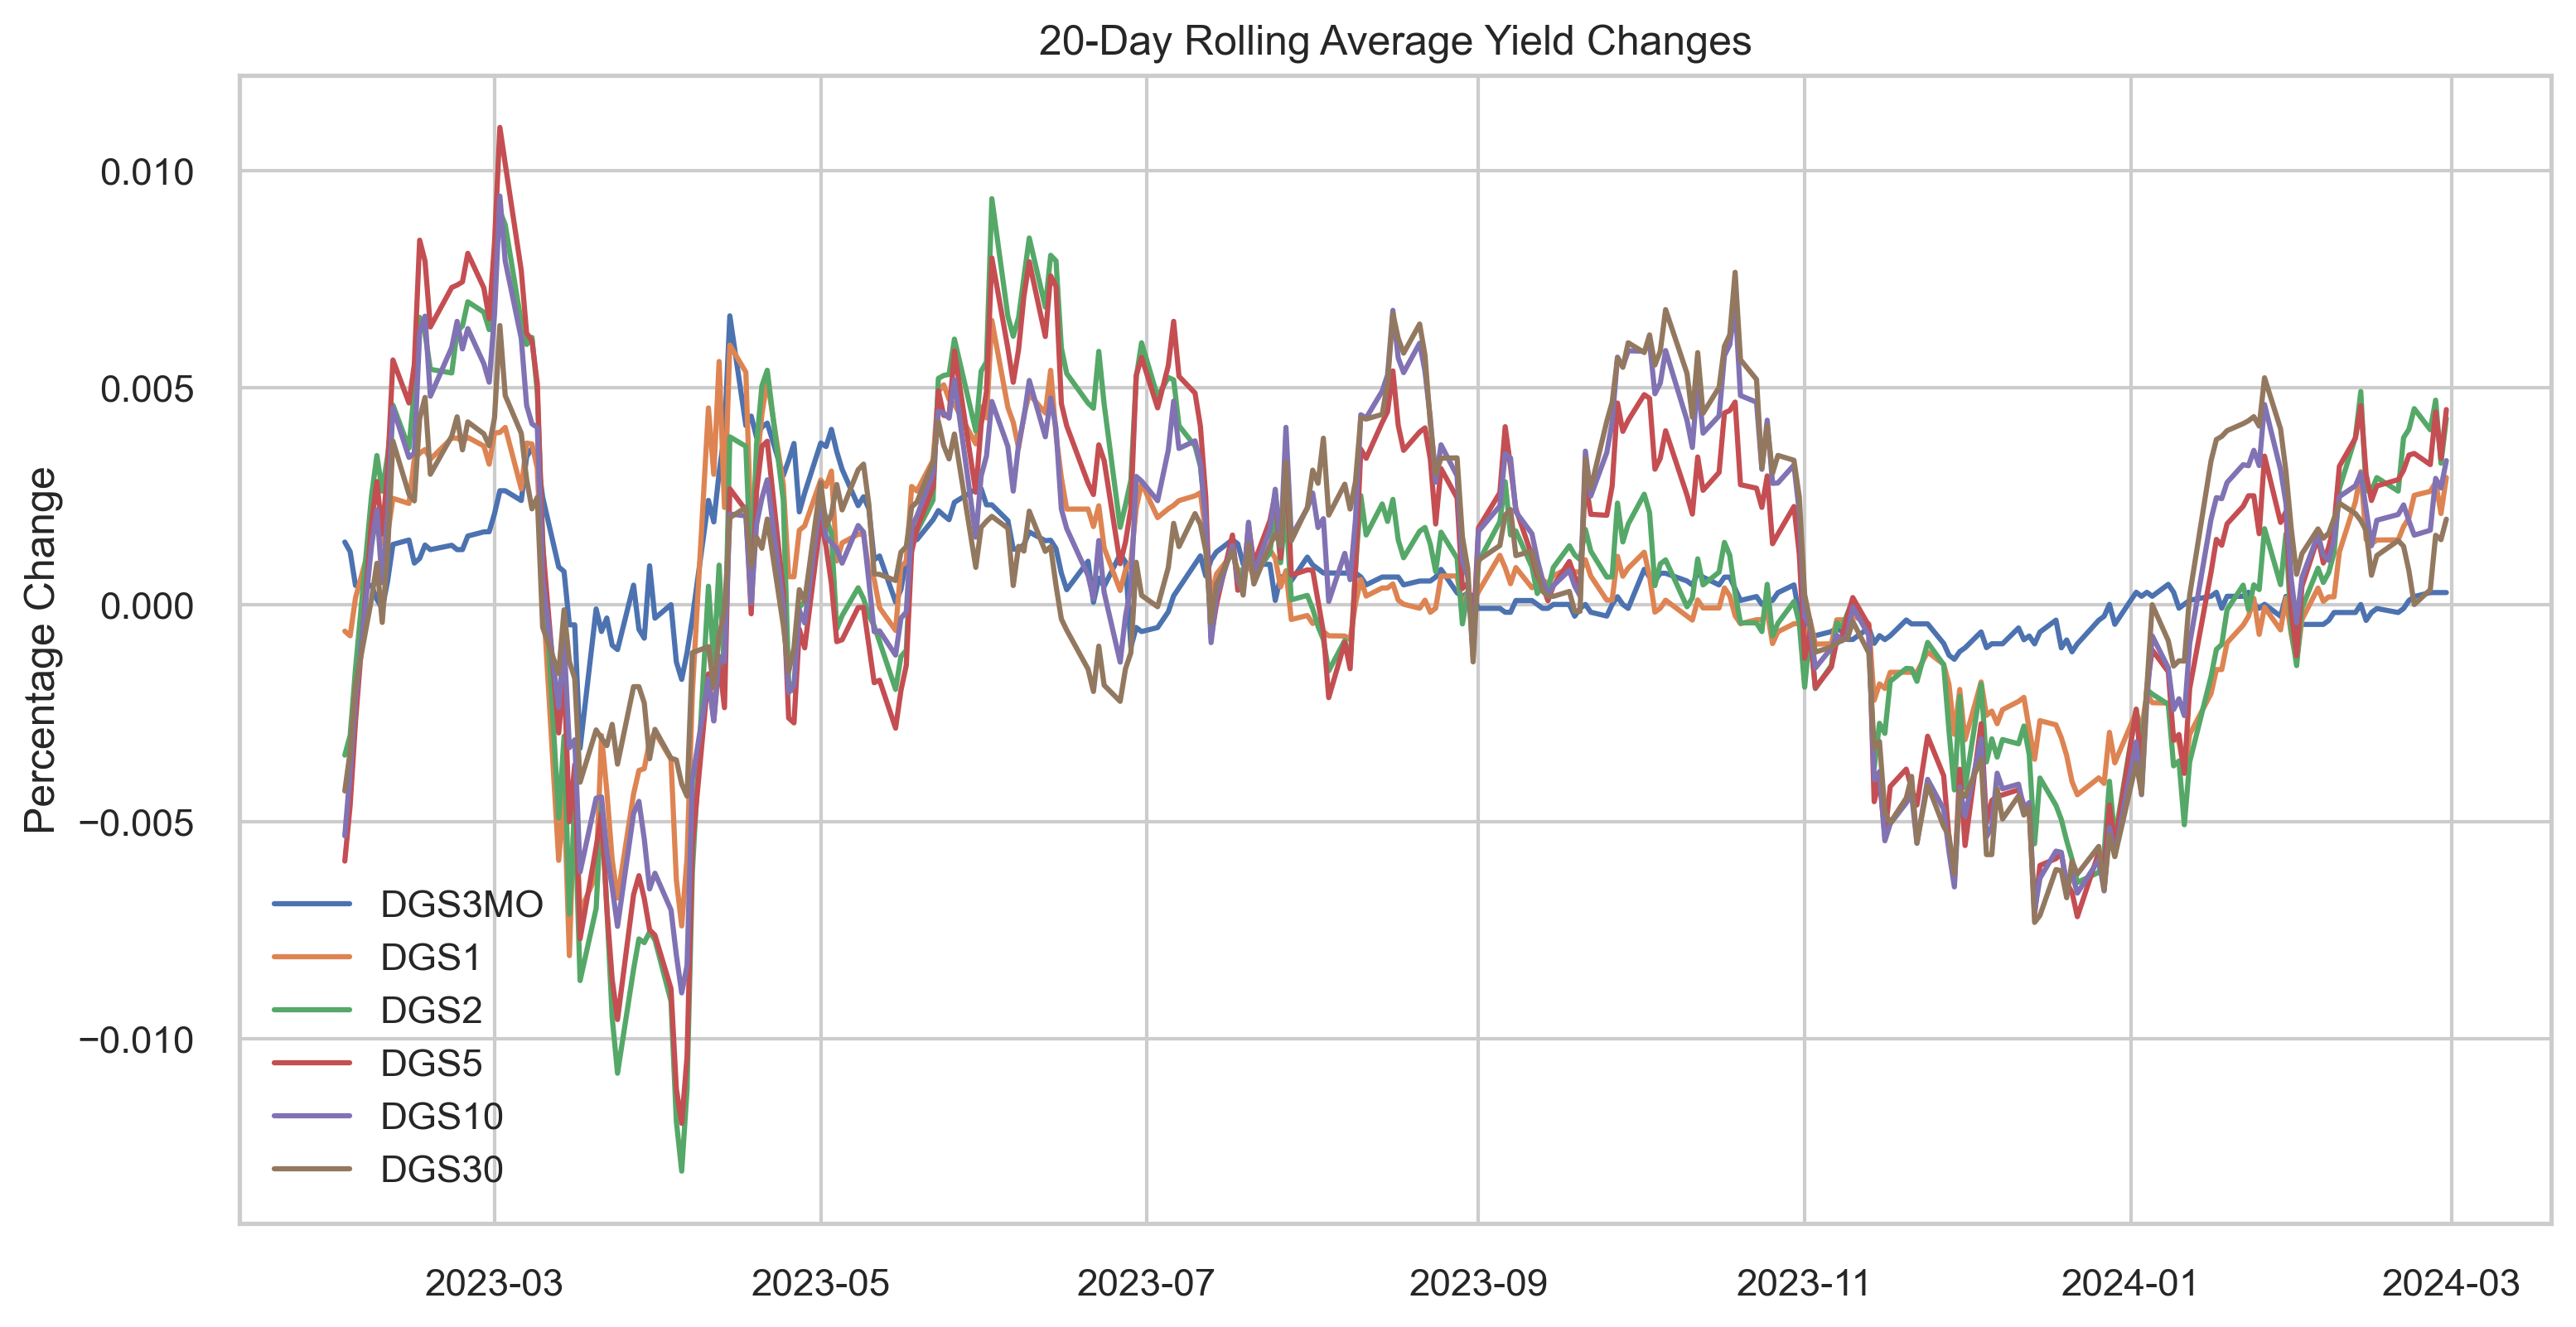
\includegraphics[width=0.8\textwidth]{figures/yield_changes.png}
    \caption{20-Day Rolling Average Yield Changes}
    \label{fig:yield_changes}
\end{figure}

\begin{figure}[H]
    \centering
    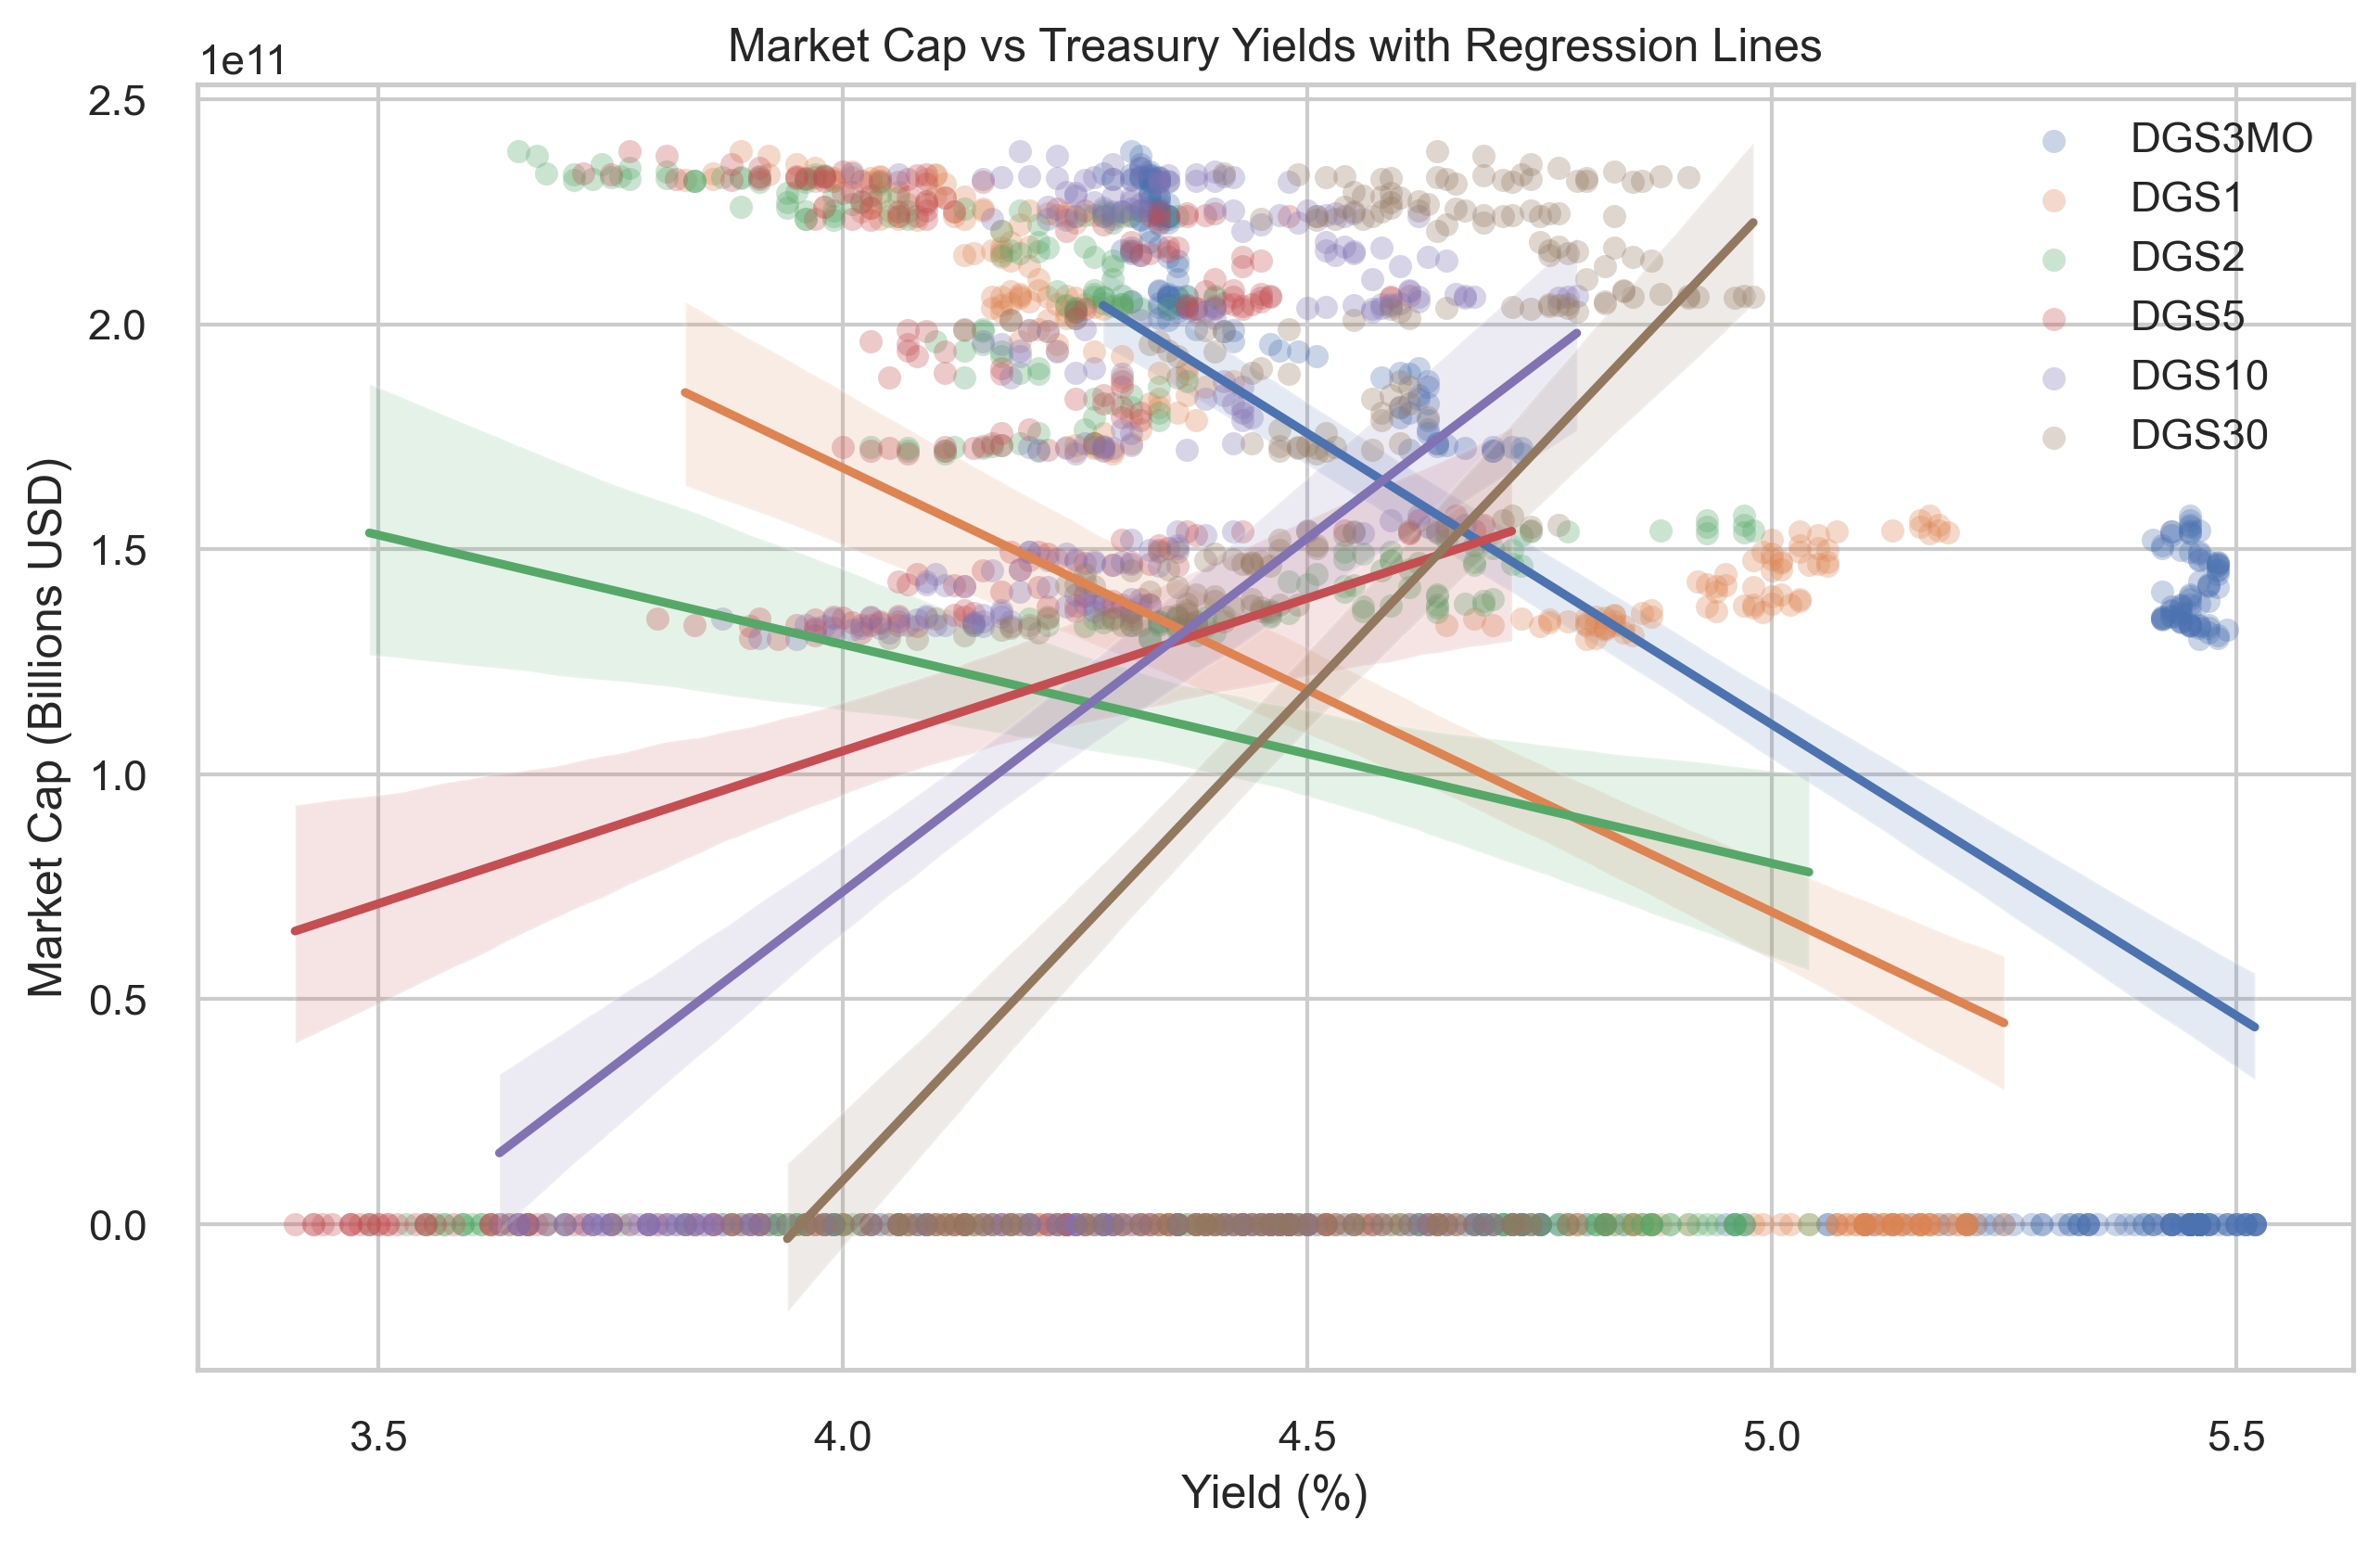
\includegraphics[width=0.8\textwidth]{figures/market_cap_vs_all_yields.png}
    \caption{Market Cap vs Treasury Yields with Regression Lines}
    \label{fig:regression}
\end{figure}

\end{document}
